\chapter{Background}
This section will provide some details on the physics being modeled and the math behind the solvers used. In addition an
introduction to modern parallel programming and GPGPU will be given, with special focus on CUDA.

% ==Particle-In-Cell Codes== %
\section{Particle-In-Cell Codes}
Particle simulations attempt to model the behavior and interactions of particles and their forces, with applications in
for example fluid dynamics or studies of plasma, they tend to be very compute intensive. One type of simulations is
called Particle-in-cell codes.

Particle-in-cell simulations consist of finding the electrical charge distribution resulting from the particle charges,
solving the field to find the electrical potential, and move the particles based on the resulting electrical force and
their current velocity. The simulation is discrete in both time and space and sufficient resolution in either is
necessary to avoid aliasing, and properly model physical phenomena such as plasma wave oscillation.

% Subject of simulation %
\subsection{Subject of simulation}
The simulation models the behavior of charged particles in an electric field. In some PIC simulations a magnetic field
is present as well, but in this project the magnetic field is assumed to have no effect. Particles are modeled with
charge, mass, position and velocity.

% Equations %
\subsection{Discrete Model Equations}
The following equations form the basis of the simulation. The simulation procedure can be derived from these equations,
as seen below. For further detail on these equations see chapter 3 of \cite{elster94}. The only major difference is that
this explanation is given with three dimensional space.
\begin{equation} \label{eq:dm1} \nabla^2\Phi = -\frac{\rho}{\epsilon _0} \end{equation}
\begin{equation} \label{eq:dm2} \mathbf{E} = -\nabla\Phi \end{equation}
\begin{equation} \label{eq:dm3} \frac{dv}{dt} =\frac{q\mathbf{E}}{m} \end{equation}
\begin{equation} \label{eq:dm4} \frac{dx}{dt} = v \end{equation}

%%
\subsubsection{Poisson's equation}
Poisson's equation is a \emph{partial differential equation} (PDE) with uses in various disciplines, and specifically electrostatics.
The general form of the equation is $\Delta\phi = f$, which in euclidean space is equal to $\nabla^2\phi = f$. In 3D
Cartesian coordinates this becomes $\frac{\partial ^2\phi}{\partial ^2 x} + \frac{\partial^2\phi}{\partial ^2 y} + \frac{\partial ^2\phi}{\partial ^2 z}= f$.

The form found in equation \ref{eq:dm1} stems from Maxwell's equations, specifically Gauss's law for electricity. In
differential form written as
$$\nabla \cdot \mathbf{D} = \rho_f$$
the equation states that the divergence of the electric displacement field $\mathbf{D}$ is equal to the free charge
density $\rho_f$. With the assumption of no polarization or bound charges we have that
$$\mathbf{D} = \epsilon_0\mathbf{E}$$
Combining these leads us to
\begin{equation} \label{eq:poisson1} \nabla \cdot \mathbf{E} = \frac{\rho_f}{\epsilon_0} \end{equation}
We assume there is no changing magnetic field present, in which the Maxwell-Faraday Equation gives us
$$\nabla \times \mathbf{E} = -\frac{\partial\mathbf{B}}{\partial t}=0$$
and in turn equation \ref{eq:dm2}:
$$\mathbf{E}=-\nabla\Phi$$
Inserting this into equation \ref{eq:poisson1} we get:
$$\nabla \cdot \nabla \Phi = -\frac{\rho_f}{\epsilon_0}$$
or
$$ \nabla^2\Phi = -\frac{\rho_f}{\epsilon _0}$$
and in 3D form
$$\frac{\partial ^2\Phi}{\partial ^2 x} + \frac{\partial^2\Phi}{\partial ^2 y} + \frac{\partial ^2\Phi}{\partial ^2 z}= -\frac{\rho_f}{\epsilon _0}$$

By solving this equation using a 3D PDE solver we can find the electric potential $\Phi$ given the distribution of
electric charge $\rho_f$. This form of Poisson's equation is also known as Poisson's equation for electrostatics.

%%
\subsubsection{Electrical force from Potential}
Given the electric potential field $\Phi$ we want to determine the electrical force on a particle at position $p$. Using
equation \ref{eq:dm2} we can find the electric field $\mathbf{E}$
$$ \mathbf{E} = -\nabla\Phi $$
which is related to the electric force by
$$ \mathbf{F}_e = q\mathbf{E}$$

\paragraph{Discretized}
We can determine the field strength at each grid vertex using first order finite differences differences in each direction:
$$ \mathbf{E}_x(i, j, k) = -\frac{\Phi(i+1, j, k) - \Phi(i-1, j, k)}{h_x} = \frac{\Phi(i-1, j, k) - \Phi(i+1, j, k)}{h_x}$$
$$ \mathbf{E}_y(i, j, k) = \frac{\Phi(i, j-1, k) - \Phi(i, j+1, k)}{h_y} $$
$$ \mathbf{E}_z(i, j, k) = \frac{\Phi(i, j, k-1) - \Phi(i, j, k+1)}{h_z} $$
To find the electrical force on a particle we then need to interpolate the field strength at its position from its cell
vertices (see figure \ref{fig:trilinear}), and divide by the particle's charge.

%%
\subsubsection{Acceleration and velocity from Electrical force}
Given the force exerted on a particle we can use Newton's laws of motion to determine the effect on
it's velocity and position. We know that the particle's acceleration is
$$\mathbf{a} = \frac{\mathbf{F}}{m}$$
$$\mathbf{a} = \frac{d\mathbf{v}(t)}{dt}$$
$$\mathbf{v} = \frac{d\mathbf{x}(t)}{dt}$$

\paragraph{The leap frog method}
The particle's position and velocity is updated by integrating these equations, and in order to ensure a stable
simulation a leap frog integration method is used. By letting the position and velocity updates occur with half a
time-step's delay between, they "leap" over each other, resulting in a method more stable than the Euler method for
oscillations. The resulting discrete equations are:
$$v_{n+^{\!1}/_2} = v_{n-^{1\!}/_2} + \frac{\mathbf{F}(x, y, z)}{m}\cdot \Delta t$$
$$p_{n+1} = p_n + v_{n-^{1\!}/_2}\cdot \Delta t$$

\begin{figure}[!htbp]
	\centering
	\includegraphics[width=0.65\textwidth]{figure/leapfrog}
	\caption[Leap frog illustration]{An illustration showing how velocity and position are updated in a way causing them to "leap frog" over each
	other. Shown in transparent red are arrows illustrating $v_n$.}
	\label{fig:leapfrog}
\end{figure}

\subsubsection{Finding the charge distribution $\rho_f$}
In order to find the charge density on the grid we interpolate a particle's contribution to charge on it's neighboring
vertices, similarly to how the electrical field strength is interpolated. A particle's contribution to a vertex is
inversely proportional to their distance. The trilinear interpolation used is illustrated in figure \ref{fig:trilinear}

% Procedure %
\subsection{Procedure}
\begin{enumerate}
	\item Find charge density by accumulating particle charges on the grid.
	\item Solve for electrical potential using equation \ref{eq:dm1}.
	\item Derive electric field strength at all grid vertices from potential, using finite differences (\ref{eq:dm2}).
	\item Update particles:
	\begin{enumerate}
		\item Determine electrical field strength at particle position by trilinear interpolation of current cell vertex values.
		\item Using relation between acceleration, electrical force and electrical field strength, update particle velocity (\ref{eq:dm3}).
		\item Update particle position using updated velocity (\ref{eq:dm4}).
	\end{enumerate}
\end{enumerate}

% ==Solvers== %
\section{Solvers}\label{sec:background-solvers}
In order to handle different boundary conditions two different solvers have been implemented, one using the \emph{Fast Fourier
Transform}, the other based on \emph{Successive Over-Relaxation}. These are the same described by Elster in section 3.3 of \cite{elster94}.

% FFT %
\subsection{Fast Fourier Transform}
The fast Fourier transform is an efficient implementation of a discrete Fourier transform, which calculates a spectral
transform of a discrete signal. With extremely broad application, the FFT is known as one of the most important algorithms
in computer science today. A brief explanation of the FFT and it's background will be given.

\subsubsection*{Fourier Transform}
From a mathematical viewpoint the Fourier transform is an expression of a function of time as a function of frequency.
Related to the Fourier series, where a function can be approximated by a sum of sine and cosine terms, the Fourier
transform is similar to an infinite series, and the sum is replaced by an integral:
\begin{equation}
	\label{eq:ft}
	\hat{f}(\xi) = \int_{-\infty}^\infty f(x) e^{-2\pi i x \xi} dx
\end{equation}
Although equation \ref{eq:ft} shows a one dimensional transform this generalizes to any number of dimensions.

\subsubsection*{DFT}
A DFT shares most properties with the continuous Fourier transform, apart from being discrete in both input and output.
While the continuous transform ia a mathematical operation, the DFT has practical applications in ex. signal processing.
Compare equation \ref{eq:ft} for the Fourier transform with \ref{eq:dft} for the DFT:
\begin{equation}
	\label{eq:dft}
	X_k = \sum_{n=0}^{N-1} x_n \cdot e^{- 2\pi i k n / N}, k \in \mathbb{Z}
\end{equation}
$X$ is a length $N$ array of complex values, where each element $X_k$ represents one frequency bucket. A one dimensional DFT
 can be seen as finding the frequency distribution of the input signal, and as such each output element depends on the
 entire input array. The number of operations required for a full transformation is therefore $O(N^2)$.


\subsubsection*{Cooley-Tukey FFT algorithm}
The Cooley-Tukey FFT is of the most frequently used fast Fourier transforms. The FFT is an improvement over the DFT,
dividing a transform into a composite of smaller transforms recursively. The following example will divide by 2 (radix-2 FFT),
but any small prime can be used (mixed-radix FFT), letting the algorithm handle any length $n=2^a \cdot 3^b \cdot 5^c...$
The sum in equation \ref{eq:dft} is split into even and odd sums:
\begin{align*}
	X_k &= \sum_{n=0}^{N/2-1} x_{2n} \cdot e^{\frac{- 2\pi i k (2n)}{N}} + \sum_{n=0}^{N/2-1} x_{2n+1} \cdot e^{\frac{- 2\pi i k (2n+1)}{N}}\\
	X_k &= \sum_{n=0}^{N/2-1} x_{2n} \cdot e^{\frac{- 2\pi i k (2n)}{N}} + e^{\frac{- 2\pi i k}{N}} \cdot \sum_{n=0}^{N/2-1} x_{2n+1} \cdot e^{\frac{- 2\pi i k (2n)}{N}}\\
	X_k &= \sum_{n=0}^{N/2-1} x_{2n} \cdot e^{\frac{- 2\pi i k n}{N/2}} + e^{\frac{- 2\pi i k}{N}} \cdot \sum_{n=0}^{N/2-1} x_{2n+1} \cdot e^{\frac{- 2\pi i k n}{N/2}}
\end{align*}
	We can see that each sum corresponds to the transform of the odd and even parts of the input, with a common twiddle
	factor $e^{\frac{- 2\pi i k n}{N/2}}$. Since the input is assumed to be periodic either sum has the same value for $k=m$
	and $k=m+\frac{N}{2}$. Expressing the even sum as $C_k$ and the odd as $D_k$ we get:
\begin{align*}
	X_k &= C_k + e^{\frac{- 2\pi i k}{N}} \cdot D_k\\
	X_{k+\frac{N}{2}} &= C_{k+\frac{N}{2}} + e^{\frac{- 2\pi i}{N} (k+\frac{N}{2})} \cdot D_{k+\frac{N}{2}}\\
		&= C_k + e^{\frac{- 2\pi i}{N}k}\cdot e^{\frac{-2\pi i}{N}\cdot\frac{N}{2}} \cdot D_k\\
		&= C_k + e^{\frac{- 2\pi i}{N}k}\cdot e^{-\pi i} \cdot D_k\\
		&= C_k + e^{\frac{- 2\pi i}{N}k}\cdot (-1) \cdot D_k\\
		&= C_k - e^{\frac{- 2\pi i}{N}k}\cdot D_k
\end{align*}
 By reusing the values the number of computations is drastically reduced compared to the plain DFT.

\subsubsection*{Performance}
A main reason that the FFT has seen such widespread use is it's performance, sporting an $O\left(n\cdot log(n)\right)$
complexity, compared to the DFT at $O(n^2)$. As long as the dimensions of the input are multiples of small primes,
ideally a power of 2, the FFT is very efficient. For a number of reasons, ex. data alignment, this is often the case.

\subsubsection*{Properties/Issues}
An issue with the Fourier transform is aliasing, which may occur when there are signals in the input with frequencies
higher than the resolution of the transform. The result is that the transform interprets the samples from the signal at
a lower frequency. See figure \ref{fig:aliasing} for an illustration. The \emph{Nyquist theorem} states that to avoid
aliasing a sampling frequency at least twice the highest input frequency is needed. In cases where the highest input
frequency is unknown this can be hard to ensure, but aliasing will often be clearly visible in the output, for example as
procedural noise. Avoiding aliasing is one reason we want to maximize grid resolution in the implementation, since the
sampling frequency is the inverse of grid length in each direction, $f_x = n_x^{-1}$.
\begin{figure}[!htbp]
	\centering
	\includegraphics[width=\textwidth]{figure/aliasing}
	\caption[Aliasing]{An illustration of how a high frequency signal (green) can be misrepresented as a low frequency one (blue) due to insufficient sampling frequency.
	Samples shown as red circles.}
	\label{fig:aliasing}
\end{figure}

% SOR %
\subsection{SOR solver}
Successive over-relaxation is a scheme for iterative solvers, using a relaxation factor as a weight to ensure either
faster convergence. One assumes that the solution "lies further ahead", by weighting the value of neighboring
elements higher at the cost of an element's previous value.

\subsubsection*{System of linear equations}
A system of linear equations is the problem of finding $n$ unknowns $\mathbf{x}$, given $m$ linear equations on the form
$ a_{i1}x_1 + a_{i2}x_2 + a_{i3}x_3 + ... + a_{in}x_n = b_i $. In practice we are interested in solving systems where
$n \equiv m$ meaning there exists one unique solution. The simplest such system is $ax=b$, which is trivial in nature.
Practical applications can have systems with several thousand variables. Our problem can be represented as a two
dimensional system, with a relation between values in either direction.

\subsubsection*{The Jacobi method}
Among the most famous iterative linear solvers for systems of linear equations are the Jacobi and Gauss-Seidel methods.
Brief explanations of both follow. Assume a systen of linear equations:
\begin{align*}
	A \mathbf{x} &= \mathbf{b}\\
\intertext{A is split into a diagonal and remainder matrix.}
	A &= D+R\\
	A\mathbf{x} &= (D+R)\mathbf{x} = \mathbf{b}\\
	D\mathbf{x} &= \mathbf{b} - R\mathbf{x}\\
	\mathbf{x} &= D^{-1}(\mathbf{b} - R\mathbf{x})\\
\intertext{Iteration $n$ updates an element using the equation:}
	\mathbf{x}^{(n+1)} &= D^{-1}(\mathbf{b} - R\mathbf{x}^{(n)})\\
\end{align*}
Pseudocode using a 5 point stencil on a 2D matrix:
\begin{lstlisting}
while (err > threshold):
	for all i, j:
		updated[i, j] =
				(old[i-1, j] + old[i+1, j] + old[i, j-1] + old[i, j+1])/4
		
		err_ij = abs(updated[i,j] - old[i,j])
		if (err_ij > err):
			err = err_ij
\end{lstlisting}

\subsubsection*{Gauss-Seidel} 
Because a value depends on all neighboring old values, updates have to be written to a new matrix, resulting in a $2n$
storage requirement. The Gauss-Seidel method improves upon this by replacing reads to old values with updated ones, thus
allowing in-place updates. In addition this is shown to converge faster. Using the same matrix A,
\begin{align*}
	A &= L + D + U\\
\intertext{A is divided into lower triangle, diagonal, and upper triangle matrices.}
	A\mathbf{x} = (L + D + U)\mathbf{x} &= \mathbf{b}\\
	(L+D)\mathbf{x} &= \mathbf{b}-U\mathbf{x}\\
	\mathbf{x} &= (L+D)^{-1}(\mathbf{b}-U\mathbf{x})\\
\intertext{And as for Jacobi an element is updated as}
	\mathbf{x}^{(n+1)} &= (L+D)^{-1}(\mathbf{b}-U\mathbf{x}^{(n)})\\
\end{align*}
and pseudo-code for the same problem:
\begin{lstlisting}
while (err > threshold):
	for all i, j:
		updt[i, j] =
				(updt[i-1, j] + old[i+1, j] + updt[i, j-1] + old[i, j+1] )/4
		
		err_ij = abs(updated[i,j] - old[i,j])
		if (err_ij > err):
			err = err_ij
\end{lstlisting}

This way no subsequent calculations use $old[i, j]$ and updated $updt$ values can be written to the $old$ matrix. Gauss-Seidel
is therefore a more storage efficient method, important for large problems, and memory bound systems.

\subsubsection*{Over-relaxation}
A variant of Gauss-Seidel, successive over-relaxation has a minor modification which tends to result in faster convergence.
By using a weight $\omega$ (the \emph{relaxation factor}), the old value is used to either speed up convergence, or prevent divergence:
\begin{align*}
	A &= L + D + U\\
	(L + D + U)\mathbf{x} &= \mathbf{b}\\
	\omega(L + D + U)\mathbf{x} &= \omega\mathbf{b}\\
	\big[\omega L+ (\omega + 1 - 1)D\big]\mathbf{x} &= \omega\mathbf{b}-\omega U\mathbf{x}\\
	(\omega L + D)\mathbf{x} &= \omega\mathbf{b}-\big[\omega U + (\omega-1)D\big]\mathbf{x}\\
	\mathbf{x} &= (\omega L+D)^{-1}(\omega\mathbf{b}-\big[\omega U + (\omega-1)D\big]\mathbf{x})\\
	\mathbf{x}^{(n+1)} &= (\omega L+D)^{-1}(\omega\mathbf{b}-\big[\omega U + (\omega-1)D\big]\mathbf{x}^{(n)})\\
\end{align*}
\begin{lstlisting}
while (err > threshold):
	for all i, j:
		temp = (updt[i-1, j] + old[i+1, j] + updt[i, j-1] + old[i, j+1] )/4
		updt[i, j] = (omega-1) * old[i, j] + omega * temp
		
		err_ij = abs(updated[i,j] - old[i,j])
		if (err_ij > err):
			err = err_ij
\end{lstlisting}

The value of $\omega$ is used to control the influence the old value has on the new. $\omega = 1$ is the same as
Gauss-Seidel, $\omega = ^1\!/_2$ is to take the average of the old and updated values, while $\omega = 2$ would result in $ new = 2\cdot updated - old$.
For $\omega < 1$ change between iterations is diminished, and gives a lower chance of divergence. $\omega > 1$ places
more focus on neighboring values, and may speed up convergence. We want to speed up convergence, and good choice for
$\omega$ has been shown to lie around $1.78$. 

\subsubsection*{Parallelized - Red-Black coloring}
\label{sec:red-black}
A problem with the Gauss-Seidel method is the dependency between an update and those preceding it. Because $updated[i]$
depends on $updated[i-1]$, these cannot be calculated in parallel. The Jacobi method however has no dependencies to elements
from the same iteration, but cannot be done in-place. We can get the best of both worlds however, using a Red-Black
Jacobi method. By updating every other element in parallel, we avoid read-write conflicts, and no dependencies between
elements being updates, see figure \ref{fig:red-black}.

\begin{figure}[!htbp]
	\centering
	\includegraphics[width=0.6\textwidth]{figure/sor-red-black}
	\caption[Red-black ordering]{An example of 2D red-black coloring of a matrix. By first updating black, and then the red elements,
	calculations can be done in parallel, and in-place. As seen with the green stencil, the center element is only dependent on the its neighboring black elements, not on red ones.}
	\label{fig:red-black}
\end{figure}

% ==Parallel Computing== %
\section{Parallel Computing}
Parallel computing may refer to any form of processing in which multiple operations are performed concurrently. This can
range from vectorizing instructions to running ten thousands of threads on thousands of nodes on a supercomputer. A
short introduction to the history and motivation behind parallel computing will be given, as well as a measure of
performance for parallel computing.

\paragraph{Moore's law, limits of single core processing, and the rise of multi-core}
Well known to every computer scientist, Moore's law described the consistent increase in processing power since the
1970s. Performance increased along with transistor density, and was observed to double approximately every two years.
As long as performance could be increased by simply building a faster processor, interest in multi-core computing was
limited.
Three factors became readily visible during the early 2000s:
\begin{itemize}
	\item{The Memory Wall}
	Processor speeds increased faster than memory speeds, making it harder to hide memory latency. The result was that
	further increases in CPU clock speed would be lost waiting for memory.
	\item{The ILP Wall}
	While instruction level parallelism (ILP) had been used to hide the growing disparity between CPU and memory clock
	speed, it became harder to extract further instruction level parallelism from a single stream of instructions.
	\item{The Power Wall}
	$$U_{CPU voltage} = O(f_{CPU frequency})$$
	$$P_{CPU power consumption} = O(V^2_{CPU voltage})$$
	Because of these relationships, and the fact that CPU clock frequency has been doubling yearly, and number of
	transistors steadily increasing, CPUs were consuming a lot of power, and becoming very hot dissipating this energy.
	While the increase in voltage has been mitigated somewhat by the shrinking die size, the small transistors and low
	voltage causes issues like subthreshold leaking and electromigration to become more prominent. 
\end{itemize}
The result is that the cost of increasing performance while avoiding the power wall is too great, considering that
memory latency is the bottleneck.

Because of these issues the industry has shifted to multi-core computing as a way of further increasing performance. By
creating chips consisting of several smaller simpler processors rather than one large complex one, power consumption
and manufacturing costs is decreased, at the cost of being harder to program.

Another solution has been to offload work to hardware accelerators, such as graphics cards. This method, known as GPGPU
will be explained in more detail below.

\paragraph{Amdahl's law, Gustafson's law}\label{sec:background-speedup}
With the advent of parallel computing a new measure of performance is needed. while single core processing has a maximum
performance equal to $IPS = f_{clock} \cdot IPC$, the number of instructions per second is equal to the number of
instructions per clock cycle times the clock frequency. Assuming a fully parallelizable problem, the performance should
scale with the number of course, $IPS = n_{cores} \cdot f_{clock} \cdot IPC$. In reality however, not all parts of a
problem are easily parallelizable, often some setup or preprocessing has to be done sequentially. Because of this we
need a measure dependent upon the number of processors utilized, and the portion or the problem that is parallelizable.
In particular we want a measure of the speedup using $n$ processors instead of one, based on the formula:
$$S_n = \frac{T_1^{\,execution\,time}}{T_n^{\,execution\,time}}$$

\emph{Amdahl's law} gives an intuitive formula for the speedup of a program running on $n$ processors where $P_{sequential}$
is the sequential fraction of the execution time:
$$ T_n = T_1 \cdot (P_{sequential} + \frac{P_{parallel}}{n}) $$
$$ S_n = \frac{T_1}{T_n} = \frac{T_1}{T_1 \cdot (P_{sequential} + \frac{P_{parallel}}{n})} = \frac{1}{P_{sequential} + \frac{P_{parallel}}{n}}$$
This formula is useful in finding the potential speedup when parallelizing a sequential program, but as is evident, the
sequential part will quickly dominate the parallel part. By setting $n = \infty$ the formula becomes $S_\infty = \frac{1}{P_{sequential}}$,
and for a program with a 20\% sequential part the maximum speedup is 5. With $n=8$ this same problem would get a speedup
of $S_8 = \frac{1}{0.2 + \frac{0.8}{8}} = 1 / 0.3 = 3.33$, and with 16 cores the speedup would be $S_16 = 4$. Clearly
this does not scale well, and GPU computing with thousands of cores makes little sense.

The answer given in \emph{Gustafson's law} is that the approach to parallelizing the problem is wrong, and instead
defines the speedup as
$$ S_n = P_{sequential} + n \cdot P_{parallel}= n - P_{sequential} \cdot (n-1) $$
The elementary difference here is an assumption that the size of the parallel part of the computation scales linearly
with the number of processors. In other words, by increasing the problem size alojng with the number of processors, we
can keep improving the speedup without getting dominated by the serial part. One could also think of this as writing a
parallel program instead of converting a serial one, allowing the workload to be optimized for parallel computing. This
is also the clue GPGPU's potential.
% ...and anything else worth mentioning. %

% ==GPGPU== %
\section{GPGPU}
\emph{General-purpose computing on graphics processing units} (GPGPU) is a fairly recent trend in parallel computing,
where programs are accelerated by running heavy computation on a graphics processing unit. Characterized by a large
number of slower, cheaper cores, graphics cards today deliver massive parallelism to a standard desktop computer at low
cost.

% History %
\subsection{History}
Traditional graphics pipelines allowed only data to pass from the CPU to the GPU, where it would be processed in several
steps, rendered, and output to some display device. Around 2001 programmable shaders enabled researchers to experiment
with GPU computing, by defining data in terms of graphics primitives. In order to alleviate some of the trouble of
programming this way, GPU-specific languages and libraries were made, hiding the shader language from the programming.
One such language was Sh \cite{libsh}.

Coinciding with the industry's shift towards multicore/parallel programming, GPUs became increasingly powerful and easier
to develop for over the next few years. From 2006 GPUs shifted from graphics-specific pipelined devices towards generic
stream processing, with increasingly powerful parallelism as well as general programmability. Today GPUs are contending
with CPUs, offering a potentially much higher performance at the cost of some generality. For parallel applications, GPUs
offer a significantly cheaper option than the CPUs required to achieve the same performance, both in terms of value and
power budget. For this reason many current supercomputers are including GPUs to increase processing power per node,
with three among the top ten having Nvidia Tesla GPUs installed\cite{top500}. Of the 500
75 use accelerator technology, with 53 using GPUs.

Take for instance the Titan supercomputer by Cray at Oak Ridge National Laboratory, which took the lead on the TOP500 list in
November 2012, and uses Nvidia Tesla. Compared to their previous supercomputer Jaguar, performance increased from $2.3PF$
to $27PF$ while power increased from $7MW$ to $9MW$.\cite{nvidiasc14intro} This means more than a tenfold increase in performance at the cost
of only $1.3\times$ the power. Already ORN labs and Nvidia are cooperating to see similar scaling for their next
supercomputer Summit, aiming for a 2017 installation\cite{nvidiasc14intro}.

\subsection{Performance}
The \emph{Nvidia GeForce 8800 GTX} is a high end GPU from 2007 with a theoretical peak performance of 518.4 GFLOPS
\footnote{\url{http://www.techpowerup.com/gpudb/187/geforce-8800-gtx.html}} and a power consumption of $155W$.
A contemporary high end CPU, the \emph{Intel® Core™2 Extreme Processor QX9650} had a peak performance of $96GFLOPS$
\footnote{Assuming SSE: $4 cores \cdot 8 \frac{FLOPS}{cycle} \cdot 3.0GHz = 96GFLOPS$.} with a power consumption of
$130W$. See \url{http://ark.intel.com/products/33921/Intel-Core2-Extreme-Processor-QX9650-12M-Cache-3_00-GHz-1333-MHz-FSB}.

A high end consumer GPU in 2014, the \emph{GTX 980}, has a theoretical peak performance of $4612 GFLOPS$
\cite{maxwell},
drawing $165W$
\footnote{\url{http://www.geforce.com/hardware/desktop-gpus/geforce-gtx-980/specifications}}
and costs around 5000 NOK
\footnote{\url{https://www.komplett.no/search?q=GTX980}}.
In comparison Intel's current high end CPU, the \emph{Intel Core i7-5960X Extreme Edition}, has a theoretical peak performance of $768 GFLOPS$
\footnote{Assuming AVX and FMA: $8 cores \cdot 32 \frac{FLOPS}{cycle} \cdot 3.0GHz = 192GFLOPS$.\\See also
\url{http://www.pugetsystems.com/blog/2014/08/29/Linpack-performance-Haswell-E-Core-i7-5960X-and-5930K-594/} for a lower estimate.},
a power consumption of $140W$
\footnote{\url{http://ark.intel.com/products/82930/Intel-Core-i7-5960X-Processor-Extreme-Edition-20M-Cache-up-to-3_50-GHz}},
and a cost of ca 9500 NOK
\footnote{\url{https://www.komplett.no/intel-core-i7-5960x-extreme-edition/822376}}.

From these numbers it looks as if the GPU provides than five times the performance at half the cost, with only a
slightly higher power consumption. In reality the performance of either will be lower, and for double precision operations
the CPU performance will decrease a lot less than will the GPU's, but it is apparent that the GPU can provide relatively
cheap performance, and that the performance continues to improve. Note that the above are only estimates based on
specifications and not measured results, and that prices may vary between vendors and stores.

% ==CUDA== %
\section{CUDA}
The \emph{Compute Unified Device Architecture}, or CUDA for short, is a GPGPU computing platform. Developed by Nvidia
and introduced in 2006, CUDA is a relatively young technology, but has already seen employment in a number of applications
and research papers.

To develop for the CUDA platform one can use CUDA libraries, languages including the C/C++ and Fortan extensions and the
OpenCL framework, and compiler directives such as OpenACC/OpenMP \cite{nvidiaopenmp}.
In addition there exists third party wrappers for many other languages.

For this project the \emph{CUDA C/C++} is used, and will be reflected in the brief introduction below.
An introduction to what CUDA is by Nvidia can be found at \url{http://blogs.nvidia.com/blog/2012/09/10/what-is-cuda-2/}.
% Programming model %
\subsection{Programming CUDA}
The CUDA C/C++ has a few special features that sets it apart from standard C/C++. Most importantly, there is a
distinction between \emph{host} and \emph{device} code. Host code runs on the CPU and is responsible for calling device code. Device
code runs on the GPU, and can be recognized as functions with the \lstinline{__global__} qualifier. These functions are
known as kernels, and several instances are executed in parallel on the CUDA cores of the GPU.

Code is compiled using Nvidia's LLVM\footnote{See \url{http://llvm.org/}}-based compiler \emph{NVCC}. NVCC in turn uses
either the GNU compiler \emph{gcc} or the Microsoft Visual Studio compiler \emph{cl} to compile host code, while device
code is compiled to the \emph{ptx} assembler language \cite{nvcc}.
When the program is executed on a device the Nvidia graphics driver compiles the ptx code into a device specific binary \cite{nvptx}.

Below is an example of a CUDA kernel, and a call to this kernel:
\begin{lstlisting}
__global__ kernel(float a, float* x, float *y, float *out, int max)
{
	// Find the index of the current thread:
	int idx = blockIdx.x * blockDim.x + threadIdx.x;
	// Stay within bounds of the arrays:
	if(idx >= max)
		return;	
	// Perform computation:
	out[idx] = a * x[idx] + y[idx];
}

// Host code
int count = 20;
size_t size = count * sizeof(float)
float f = 0.25f;

float 
	*h_x, *h_y, *h_out;
	*d_x, *d_y, *d_out;
cudaMalloc(&d_x, size);
cudaMalloc(&d_y, size);
cudaMalloc(&d_out, size);

// Copy input arrays to device:
cudaMemcpy(d_x, h_x, size, cudaMemcpyHostToDevice)
cudaMemcpy(d_y, h_y, size, cudaMemcpyHostToDevice)

kernel<<<1, 32>>>(a, d_x, d_y, d_out, count);

// Copy result back to host:
cudaMemcpy(h_out, d_out, size, cudaMemcpyDeviceToHost)
\end{lstlisting}

This is a typical CUDA kernel call, although stripped of error checks and the like. We see that the host has to allocate
memory for device arrays, copy data to the device, launch the kernel and copy the result back.

In launching the kernel we see a deviation from standard C/C++ function calls, the \lstinline{<<<1, N>>>} part. These
are special parameters required by all kernels, specifying how the threads are structured, using the syntax\lstinline{<<<blocksInGrid, threadsInBlock>>>}.
Each of these accept a \lstinline{dim3} argument that specifies the length of blocks and grids in three dimensions.
Above only one value is given, specifying the x dimension while y and z default to 1.

In the kernel body we find a thread's rank within this structure though threadIdx and blockIdx, while gridDim and blockDim
correspond to the values given in \lstinline{<<<blocksInGrid, threadsInBlock>>>}. Threads are launched in \emph{warps},
groups of threads that execute concurrently on a core, and the number of threads we launch should always be a multiple
of the warp size, which is usually 32. Because of this some threads we launch may not have a designated element to work
on, and to avoid reading and writing out of bounds we check the thread index against the array size.

\begin{figure}[!htbp]
	\centering
	\includegraphics[width=0.65\textwidth]{figure/threads}
	\caption[Hierarchical structure of threads.]{The thread hierarchy in CUDA is illustrated above, with a grid containing several blocks, which themselves contain several threads.
	This configuration would be calles as \lstinline{<<<(3, 3, 1), (5, 5, 1)>>>}.}
	\label{fig:thread-hierarchy}
\end{figure}

% Memory %
\subsection{Memory}
GPU-accelerated programs tend to be very sensitive to memory accesses, and so it is very important to be conscious of
data locality when looking to optimize code. In CUDA there are three main levels of memory, global device memory, shared
block memory, and thread local memory. Using figure \ref{fig:thread-hierarchy} as an example, all threads (blue) have their
own local memory, registers, and all threads in a block (red) have access to a shared memory, while all blocks may access
global memory. The difference in memory latency between levels are in order of magnitude, so it is desirable to keep
data as close to the thread level as possible. Local and shared memory lifetime is restricted to a kernel launch, so to
keep results they have to be written to global memory.

In addition to these there is a constant memory which is read-only from device code, and texture memory which is
optimized for stencil access.

% cuFFT %
\subsection{cuFFT}
cuFFT is Nvidia's FFT framework for CUDA. It consists of the cuFFT and cuFFTW libraries, with the former designed with
GPUs in mind, and the latter serving as a porting tool for code using the well known FFTW library\footnote{\url{http://www.fftw.org/}}.
The cuFFT library is the one used in the implementation, and no further detail will be given on cuFFTW.

The library claims excellent performance for input sizes on the$n = 2^a \cdot 3^b \cdot 5^c \cdot 7^d$, and for prime
factors up to 127 it uses the efficient Cooley-Tukey algorithm. For other sizes it falls back on the less accurate Bluestein's
algorithm\cite[sec.~2.12]{cufft-doc} which handles large prime sizes better. Transforms of up to three dimensions are
supported, with a maximum of 512 million elements for single precision and 256 million elements in double precision
transforms, although limited by device memory and transform type (complex or real input etc.)\cite[sec.~1]{cufft-doc}.